\documentclass[../portafolio.tex]{subfiles}

% Solo agregue paquetes en el preámbulo de ../portafolio.tex

\begin{document}

% En esta sección, explique en detalle los siguientes aspectos:
% - Fecha de realización de la actividad
% - Título de la actividad (dentro de \section)
% - Un párrafo explicando cuál es el objetivo de la actividad
% - Nombre de personas con quien trabajó en la actividad
% - Una selección de evidencias de que usted hizo esta actividad (imágenes, códigos, respuestas a un problema teórico, etc.)
% - Una conclusión breve (qué aprendió con la actividad, qué no entendió, qué faltó trabajar, qué recomienda para futuras sesiones)

% Numero máximo de palabras en esta sección: 1000 palabras.

%%%%%%%%%%%%%%%%%%%%%%%%%%%%%%%%%%%%%%%%%%%%%%%%%%%%%%%%%%%%%%%%%%%%%%%%%%%%%%%%
\section{Ceros de Funciones}   % ejemplo: Derivadas numéricas , introducción a git , 

\hfill \textbf{Fecha de la actividad:} 09 de septiembre de 2022

\medskip


%---------------------------------------------------------------------------------
\subsection{Objetivo de la clase}
El objetivo de esta clase fue aprender a encontrar ceros de funciones a través del \textit{Método de bisección}. Los ceros de una función son los valores de $x$ cuando una función $f$ se iguala a 0, es decir, $f(x)=0$.

En este laboratorio trabajé junto a Mauricio Bastías y Jeremías Martínez.

\subsection{Desarrollo del Laboratorio}

En este laboratorio se trabajó estudiando la energía potencial de un péndulo invertido de masa $m$, largo $l$ y que está conectado a un resorte de constante $k$ a una altura $d$. La función que define su energía potencial es la ecuación \ref{e_pot_pendulo}, donde $\beta= kd^2/2mgl$ y $\theta$ representa el ángulo con respecto al eje y.

\begin{equation}
    u(\theta)=cos(\theta) + \beta sin^2(\theta) \label{e_pot_pendulo}
\end{equation}

En la primera línea del código \ref{c1cf} se definió la función $u(\theta)$, en la línea 4 se definió su derivada adelantada, pues más adelante se ocupó el método de bisección para encontrar sus raíces y en la línea 7 se creó el gráfico \ref{cerosfun}. Este gráfico se creó ejecutando un ciclo \texttt{for} para crear 10 curvas en un gráfico, donde \textit{be} es $\beta$, \textit{t} es $\theta$ y \textit{du} es la derivada de la función $u(\theta)$.

\vspace{2mm}
La gráfica de la derivada numérica de la función \ref{e_pot_pendulo} está representado en la imagen \ref{cerosfun}, donde $\theta \in [0,\frac{\pi}{2}]$. En la gráfica se logran observar 10 curvas, en la curva del extremo inferior $\beta$ toma el valor de $0.1$, luego en la curva que está sobre esta $\beta = 0.2$, la siguiente es cuando $\beta =0.3$ y así sucesivamente hasta la curva azul del extremo superior donde $\beta= 1$. 

\begin{listing}[h]
    \begin{minted}
[
frame=lines,
framesep=2mm,
baselinestretch=1.2,
bgcolor=LightGray,
fontsize=\footnotesize,
linenos
]
{python}
def u(t):
    return np.cos(t) + beta* (np.sin(t))**2
    
def du(u,t,h):
    return (u(t+h) - u(t)) / h

for beta in  np.linspace(0.1,1,10):
    plt.plot(t,du(u,t,h))
    \end{minted}
\caption{Se definió la función $u(t)$, su derivada y se creó un gráfico en el ciclo for}
\label{c1cf}
\end{listing}

Luego para encontrar los ceros no triviales se utilizo el fragmento del código \ref{c2cf}. Lo que se hizo ahí fue utilizar el método de la bisección. Después de observar que dentro del intervalo $[0$.$5,1$.$2]$ se encontraban todos los ceros, en la línea 2 y 3 del código \ref{c2cf} se eligió a $a=0$.$5$, pues para todo $u'(a)$ con $\beta>\frac{1}{2}$ resultaba que $u'(a)>0$. Similar con $b=1$.$2$, pero resultando $u'(b)<0$. Seguidamente se crea un ciclo \texttt{for} para los valores de beta mayor a $0.5$, dentro de este ciclo \texttt{for} se creó otro ciclo \texttt{for} para encontrar los ceros no triviales a través del método de la bisección. Obteniéndose así los resultados expuestos en la tabla \ref{bvstnt}. 

%\vspace{5mm}

\begin{listing}[H]
    \begin{minted}
[
frame=lines,
framesep=2mm,
baselinestretch=1.2,
bgcolor=LightGray,
fontsize=\footnotesize,
linenos
]
{python}
for beta in np.linspace(0.6,1,5):
    a=0.5
    b=1.2
    for i in range(20):
        c= 0.5*(a+b)
        condicion = du(u,a,h)*du(u,c,h)

        if condicion<0:
            b=c
        else:
            a=c
    plt.plot(c,du(u,c,h),"o", color="black")       
    \end{minted}
\caption{Fragmento de código creado para encontrar los ceros no triviales y graficarlos}
\label{c2cf}
\end{listing}

\begin{figure}[H]
    \centering
    \begin{subfigure}[b]{0.49\textwidth}
        \centering
        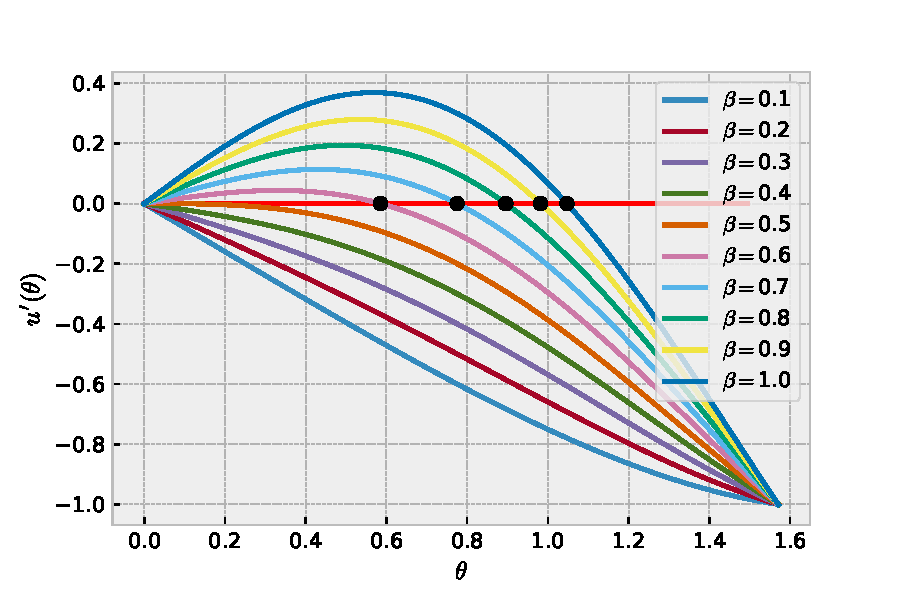
\includegraphics[width=\textwidth]{tex/img/graficoo.pdf}
        \caption{Gráfico $u'(\theta)$ v/s $\theta$.}
        \label{cerosfun}
    \end{subfigure}
    \hfill
    \begin{subfigure}[b]{0.49\textwidth}
         \centering
         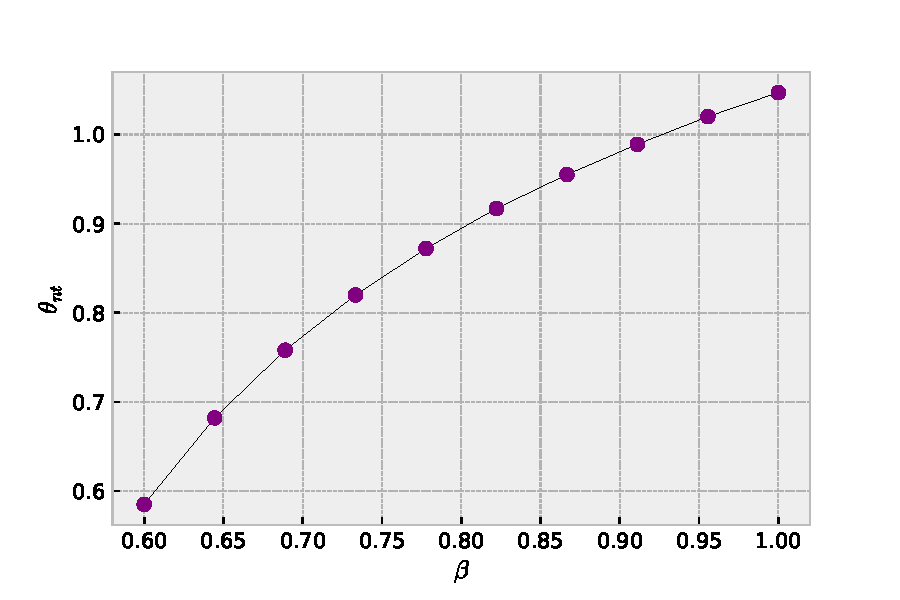
\includegraphics[width=\textwidth]{tex/img/graf_ejc.pdf}
         \caption{$\theta_{nt}$ v/s $\beta$}
         \label{ejc_graf}
     \end{subfigure}
    \caption{}
    \label{}
\end{figure}



{
\extrarowheight = -0.5ex
\renewcommand{\arraystretch}{1.75}

\begin{table}
    \centering
    \begin{tabular}{c|c}
        $\beta$  & $\theta_{nt}$ \\ \hline
        0.6 & 0.585 \\
        0.7 & 0.775 \\
        0.8 & 0.895\\
        0.9 & 0.981\\
        1 &  1.047
    \end{tabular}
    \caption{Tabla de los valores de los ceros no triviales para cada valor de beta usados en el gráfico \ref{cerosfun}.}
    \label{bvstnt}
 \end{table}   

} 

Como se logra ver en \ref{cerosfun}, las curvas cortan el eje x (sin contar el origen) solo cuando $\beta>\frac{1}{2}$.
Luego, lo  que se hizo en la línea 12 fue graficar los ceros no triviales. Estos se puede observar como puntos negros en el gráfico \ref{cerosfun}. 

En el gráfico \ref{ejc_graf} se pueden observar los ceros no triviales $\theta$ en función de $\beta$.





%\vspace{5mm}
Finalmente, se definió la segunda derivada de $u''(\theta)$ y se graficaron los puntos $u''(0)$ en función de $\beta$ para sus 10 valores quedando así el gráfico de la izquierda en la figura \ref{cerosd}. Para ello se escribió el código \ref{c3cf}.

\begin{figure}[H]
    \centering
    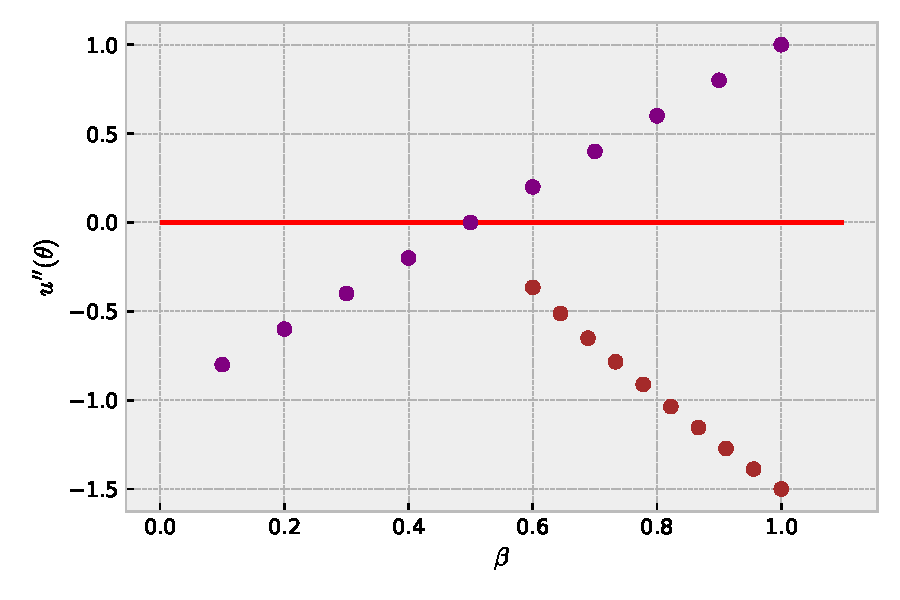
\includegraphics[scale=0.70]{ej_d.pdf}
    \caption{Los puntos morados representan $u''(0)$ con respecto a los valores de $\beta$. Por otra parte, los puntos rojizos representan $u(\theta_{nt})$ con respecto a los valores de $\beta>0.5$}
    \label{cerosd}
\end{figure}

\begin{listing}[H]
    \begin{minted}
[
frame=lines,
framesep=2mm,
baselinestretch=1.2,
bgcolor=LightGray,
fontsize=\footnotesize,
linenos
]
{python}
def ddu(u,t,h):
    return ( u(t+h) - 2*u(t) + u(t-h)) / (h**2)
    
for beta in np.linspace(0.1,1,10): #con theta igual a 0
    plt.plot(beta,ddu(u,0,h),"o")
    \end{minted}

\caption{Se definió la segunda derivada de $u$ y se creó el gráfico izquierdo de la figura \ref{cerosd}}
\label{c3cf}
\end{listing}

En el fragmento del código \ref{c3cf} se definió la segunda derivada centrada de $u$ en la linea 1 y luego a través de un ciclo \texttt{for} en la linea 4 se creó un gráfico con los valores de beta en el eje $x$ y los valores de $u''(0)$ en el eje $y$. 

\vspace{5mm}

\begin{listing}[h]
    \begin{minted}
[
frame=lines,
framesep=2mm,
baselinestretch=1.2,
bgcolor=LightGray,
fontsize=\footnotesize,
linenos
]
{python}
c_nt=[0.585, 0.682, 0.758, 0.820, 0.872, 0.917, 0.955, 0.989, 1.020, 1.047]

a= np.linspace(0.6,1,10)

for i in range(0,5):            #con los ceros no triviales
    beta= a[i]
    plt.plot(beta,ddu(u, c_nt[i], h), "o" )
    \end{minted}

\caption{Código para crear el gráfico derecho del la figura \ref{cerosd}}
\label{c4cf}
\end{listing}

También se graficaron 10 puntos de $u''(\theta_{nt})$ para los valores de $\beta > \frac{1}{2}$ quedando el gráfica de la derecha en la figura \ref{cerosd}. Para esto se redactó el fragmento de código \ref{c4cf}.
En la primera linea del código \ref{c4cf} se define una lista con los ceros no triviales relacionados a $\beta=0.6$ hasta $\beta=1$, respectivamente. Luego se creó un ciclo \texttt{for} para para graficar $u''(\theta_{nt})$ v/s $\beta$.

\vspace{5mm}
Al analizar los gráficos presentes en la figura \ref{cerosd} se puede establecer que $\theta =\theta_{nt}$ corresponde a un equilibrio inestable del sistema para todo valor de $\beta>\frac{1}{2}$, pues la segunda derivada de $u$ es negativa. Por otro lado, para $\theta=0$ el sistema está en un equilibrio inestable cuando $\beta<\frac{1}{2}$, para $\beta>\frac{1}{2}$ está en equilibrio estable, porque $u''$ es positivo, y para $\beta=\frac{1}{2}$ se encuentra en equilibrio indiferente o neutral, pues la segunda derivada es igual a cero \cite{equilibrio}.

%--------------------------------------------------------------

\subsection{Conclusiones}

En este laboratorio se trabajó encontrando los puntos de equilibrio de un péndulo invertido, para ello se debió encontrar las raíces de la derivada de la función que definía su energía potencial. La función de la energía potencial del péndulo es \ref{e_pot_pendulo}. Para encontrar los ceros no triviales de la derivada de \ref{e_pot_pendulo} se utilizó el método de la bisección y finalmente se determinaron los valores de $\theta$ para cuando correspondía a un equilibrio estable o inestable.

\vspace{2mm}
En resumen puedo decir que en el desarrollo de esta actividad aprendí a encontrar ceros de funciones usando el método de la bisección y para ello es recomendable graficar la función con anticipación para definir un intervalo $[a,b]$, tal que $f(a)\cdot f(b)<0$.

\vspace{2mm}
Al finalizar la actividad no me quedaron dudas de cómo utilizar y ni de cómo programar este método, ya que creo haberlo entendido bien. Por otra parte, me hubiera gustado haber trabajado con algún método más, pues creo que el método de la bisección no presenta una mayor dificultad aprender a usarlo y quizás nos hubiera dado tiempo para trabajar con otro método más.






\end{document}
